\section{INTRODUCTION}
\label{s:intro}

Vandalism is a problem encountered in content systems where the set of users with permission to edit is not restricted to a small set of trusted users. In Wikipedia, where the barrier to editing is particularly and intentionally low, while the need for credibility is critical, vandalism is a major concern. Vandalism that is not promptly reverted pose problems not only because it can convey misinformation and ruin the site's reputation, but also because of certain security issues. Vandalism, when left unchecked, can even be used as a vector for other malicious attacks such as directing users via external links to phishing sites or sites containing malware.

Vandalism is not a trivial problem on Wikipedia; a randomly visited page would contain vandalism with probability 0.2\%~\cite{vandalism-statistics}. Detecting and reverting vandalism is also nontrivial; 8.1\% of edits create vandalism, and 8.9\% of edits revert vandalism~\cite{changes-survey}.

Wikipedia currently uses a reactive model to vandalism, rather than a preventative model. A group of users, often self-named ``patrollers'' for vandalism, scan the list of recent changes to Wikipedia, looking for vandalism~\cite{recent}. These users then find and revert vandalism. Vandalism detection algorithms like ClueBot NG can be particularly helpful for assisting these users, as they can identify edits which are likely to be vandalism and notify patrollers of those edits. This way, the efforts of patrollers can be concentrated on a smaller group of edits which are more likely to be vandalism. Vandalism detection algorithms like ClueBot NG can also revert edits automatically if those edits are heavily suspected of being vandalism.

Vandalism detection algorithms are not always correct. In the event of a false positive (the tool detects a legitimate edit as vandalism, and reverts it) then a user can undo the revert, in which case the algorithm will leave it as-is. In the event of a false negative (the tool fails to detect and revert actual vandalism) then the page will remain vandalized until someone else notices, and reverts it manually.

\begin{figure}[t]
\centering
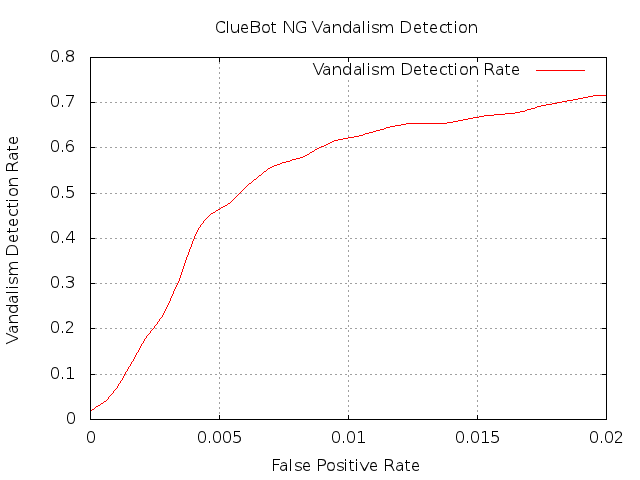
\includegraphics[width=0.7\textwidth]{figs/falsepositives-prev.png}
\vspace{-1em}
\caption{false positive rate v.s. vandalism detection rate in original \sys}
\label{f:falsepositives-prev}
\end{figure}

There are tradeoffs for each type of error; one can manipulate the threshold for declaring an edit as vandalism to reduce the number of false positives, or false negatives. In the case of \sys, the algorithm's thresholds are clearly tailored towards minimizing false positives -- the version on the sites (without our modifications) catches only 5.1$\%$ of the vandalism in the test dataset of vandalism. The particular reason for minimizing false positives is to avoid alienating users by auto-reverting their edits; new editors who have their edits auto-reverted by systems like \sys are often not aware that it was a bot which auto-reverted their edit, and can rather believe that the Wikipedia community is not welcoming of new editors, and thus stop contributing. Changing the submission and reversion process to make it more apparent and visible that algorithmic vandalism review is taking place, particularly for such new editors, may allow for a higher false positive rate to be tolerated (hence allowing more vandalism to be caught) without alienating new editors.
We define cyber vandalism as a form of activity taken up by adversaries who damage information infrastructures on the internet. There are several forms of internet vandals:

\begin{CompactItemize}
\item[1.]
Denial of Service Attacks
\item[2.]
Penetrate, hide, and collect
\item[3.]
Information Vandalism
\end{CompactItemize}

The first form of vandalism deals with adversaries trying to prevent access of certain contents to other users, disrupting either information flow (to the users) or business (for the website). The second form deals more in terms with sites that deal with money, such as paypal, amazon, etc. The third form of vandalism is the one we are most interested in controlling. We define information vandalism as any form of vandalism in an attempt to falsify, delete, or prevent accurate information on the internet. We chose Wikipedia, one of the most frequented sites of information, as our model for testing ways of preventing information vandalism.
Due to the very reason that Wikipedia defends against vandalism using a reactive model, various forms of vandalism remaining undetected have resulted in a series of humiliating incidents, including users filing lawsuits against Wikipedia for slander due to their biography pages having been vandalized~\cite{golfer-sues-wikipedia-vandalism}.

In response Wikipedia has attempted to implement a series of measures in order to alleviate vandals. We can divide them into 2 categories: editing-policy measures (ie, requiring edits to be approved, or preventing anonymous edits to certain pages), and algorithmic vandalism-detection.

Editing-policy measures that Wikipedia has put into place include semi-protecting pages that are extremely prone to vandalism (preventing anonymous users from making edits to those pages). Another editing-policy measure that hcdas been tried is Pending Changes, which requires edits by users to be approved by a special class of ``reviewers'', before reaching the site. This Pending Changes system was discontinued on the English Wikipedia after receiving mixed feedback, though it continues to be used on other wikis, such as the German Wikipedia. One part of our project proposes an alternative editing policy, Voting-Delayed Revisions, which keeps the benefits of Pending Changes without many of the problems users complained about.

Algorithmic vandalism detection began with simple rule-based systems which looked for edits that blanked pages or introduced profanity, and reverted them. Today, the state-of-the-art vandalism detection system is \sys, which uses machine learning on a corpus of labeled vandalism. Although \sys is precise, having few false positives, it is not accurate, as it misses much of the vandalism that reaches Wikipedia. The other part of our project focuses on introducing additional features to improve the effectiveness of \sys, as well as integrating \sys into our Voting-Delayed Revisions proposal to ensure that it can help prevent more vandalism from emerging to the site, than if it had simply been reverting edits.

The main contributions of this paper involves:
\begin{enumerate}
\item[1.] An editing policy that keeps the benefits of Pending Changes without many of the problems users complained about.
\item[2.] Introducing more than 20 additional features to improve the effectiveness of ClueBot NG at finding vandalism.
\item[3.] Integrating ClueBot NG into our Voting-Delayed Revision proposal to allow it to be utilized for preventing more vandalism, with lower cost for false-positives.
\end{enumerate}
